
\chapter{Gradient Descent}
\section{Model based machine learning}
There are 3 steps to this model:
\begin{enumerate}
	\item Pick a model (DT, perceptron)
	\item Pick a criterion to optimize
	\item Develop a learning algorithm
\end{enumerate}

In linear model: 
\begin{enumerate}
	\item 0 = b+ $\sum_{j=1}^{n} w_jf_j$
	\item $\sum_{i=1}^{n}1[y_y(w\cdot x_i + b) \leq 0]$ (0/1 Loss function aka the total number of mistakes)
	\item $argmin_{w,b}$ $\sum_{i=1}^{n}1[y_y(w\cdot x_i + b) \leq 0]$
\end{enumerate}

\section{Surrogate loss functions}
Minimizing the 0/1 Loss function is an NP-hard problem, because of the many local minima and any change in w can change drastically the result. Ideally we would want a convex function so to have at least one minimum.

By \textbf{surrogate loss function} we mean a loss function that provides an upper bound to the 0/1 loss function. 

\begin{itemize}
	\item 0/1 loss : $l(y,y') = 1[yy'\leq 0]$
	\item Hinge loss: $l(y,y') = max(0,1-yy')$
	\item Exponential loss: $l(y,y') = exp(yy')$
	\item Squared loss: $l(y,y') = (y-y')^2$
\end{itemize}

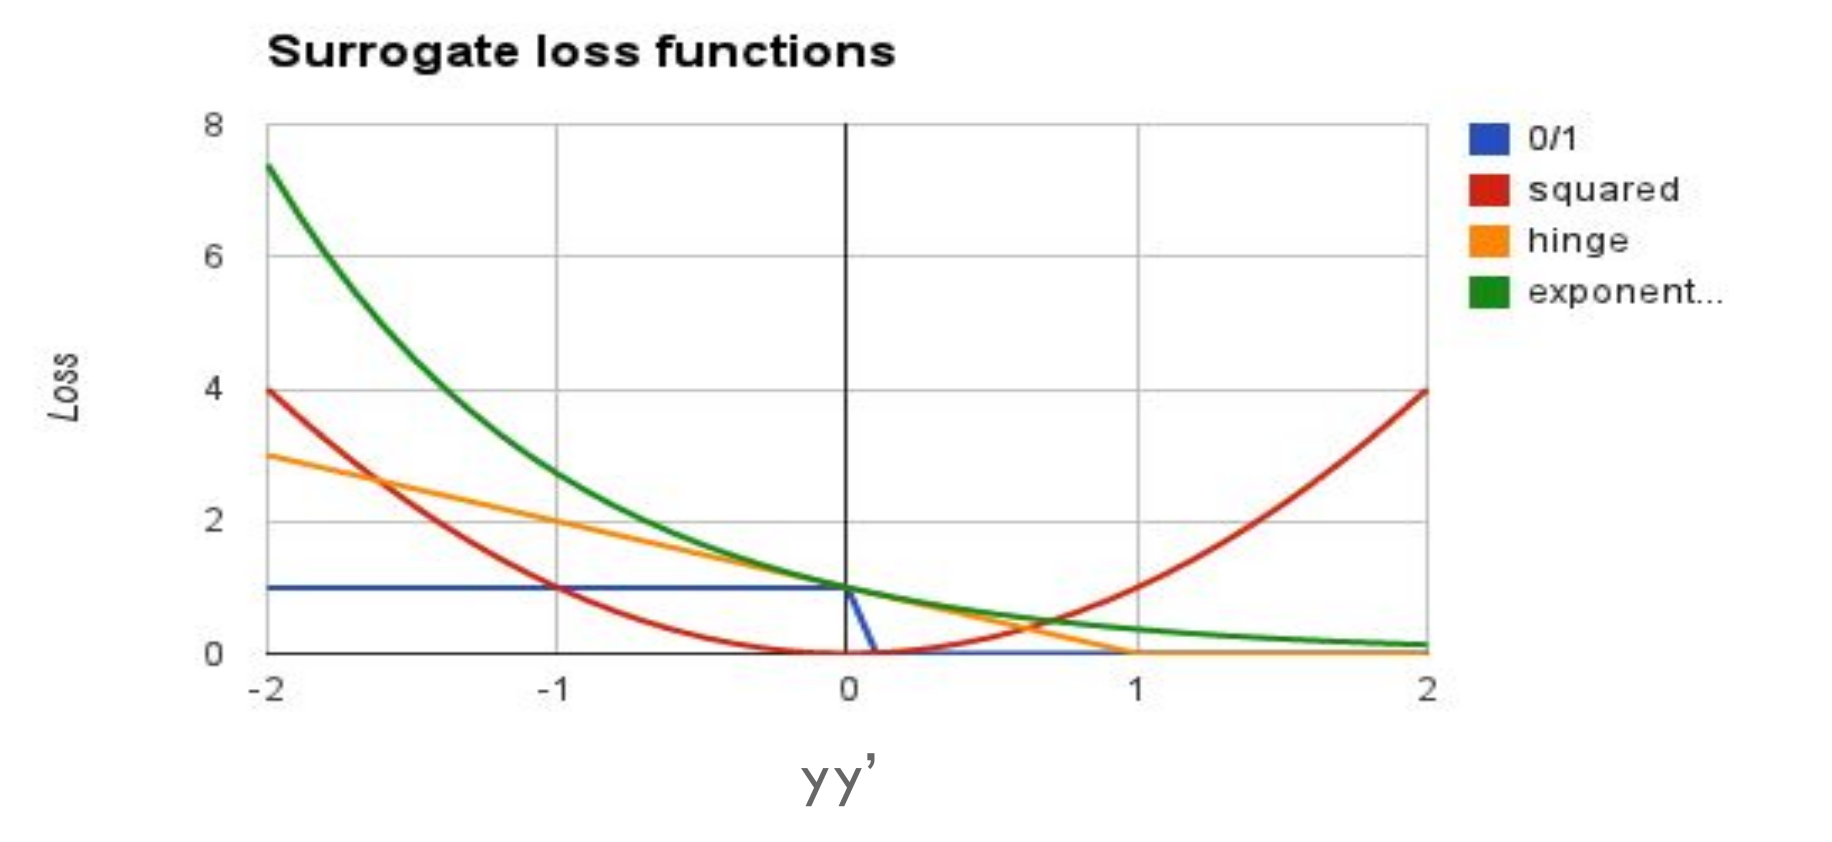
\includegraphics[scale=0.2]{surrogate}

\section{Gradient descent}
We use gradient descent to find a minimum in the function. 

The general approach is to choose a starting point $w$, calculate the derivative and move in that direction.

\[
w_j = w_j - \eta \frac{d}{dw_i}loss(w)
\]



$\eta$ is the rate at which we move and will change over time.

Since it's changing over time it can be implemented through a perceptron algorithm.

The main problem with gradient descent is local minima: 

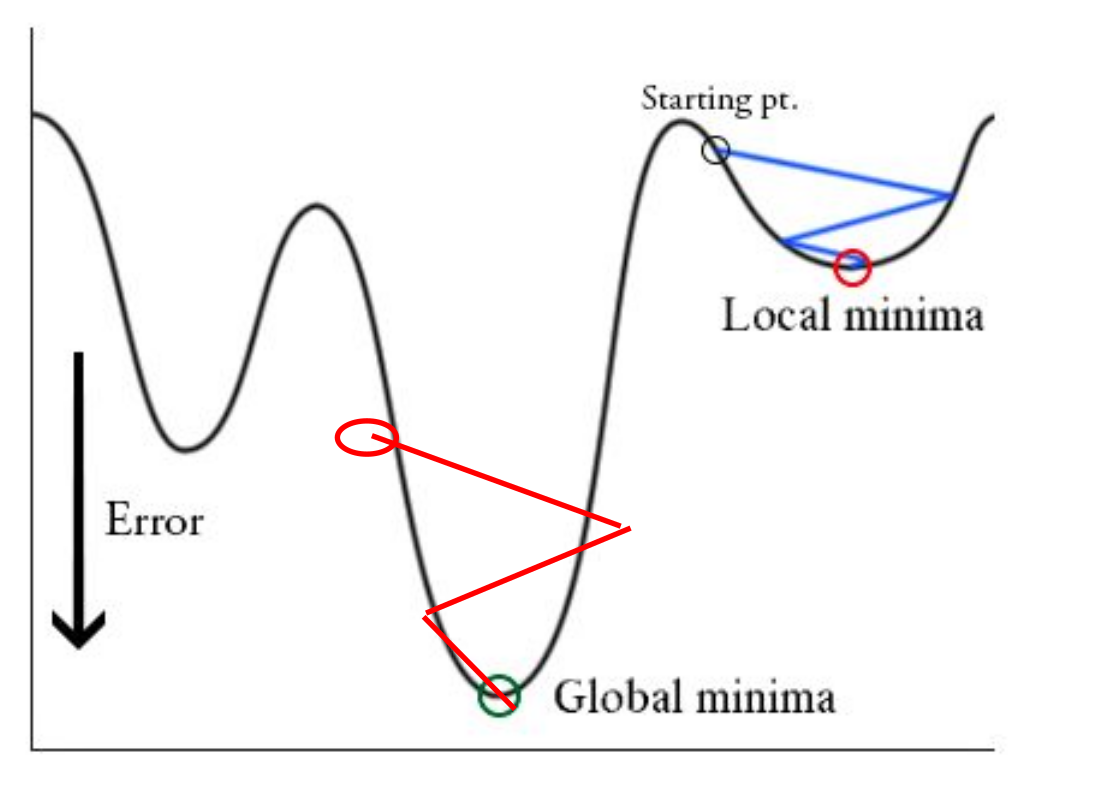
\includegraphics[scale=0.2]{local_minima}